\chapter{Dynamic Project Naming}\label{sec:project-naming}


Dynamic project naming can be achieved by creating a simple Python module that returns
a project name string in the desired format.  This concept requires a bit of background
in Python programming to achieve.  In most cases, the code required will be simple.
Complex cases will require a bit more of a Python background.  As always, 
Checkmarx Professional Services can assist with Python expertise if needed.

The project naming script is invoked with parameters that include the JSON context of the event
and a service object for interacting with the API of the SCM that generated the event.


\section{Configuration}

This section will reference the example YAML files that can be downloaded from the \cxoneflow release artifacts.
In the example YAML archive, project naming Python files are also available to provide a basic
implementation reference.  The \intlink{sec:yaml-root}{\texttt{script-path}} element
should be set to a directory where Python naming scripts have been mapped to the running \cxoneflow container.  
The directory mapping method depends on how the container is executed; one approach would be to map
a local directory to the running \cxoneflow container when creating a
\intlink{sec:container-creation}{container instance}.

With the \texttt{script-path} element configured, each service definition where the script applies
is configured with the \intlink{sec:project-naming-elements}{project naming elements}.  Figures \ref{fig:naming-yaml-adoe},
\ref{fig:naming-yaml-bbdc}, \ref{fig:naming-yaml-gh}, and \ref{fig:naming-yaml-gl} show the YAML configuration
required for custom project naming with SCM-specific scripts for Azure DevOps, BitBucket Data Center, GitHub, and
Gitlab respectively.


\begin{figure}[h]
    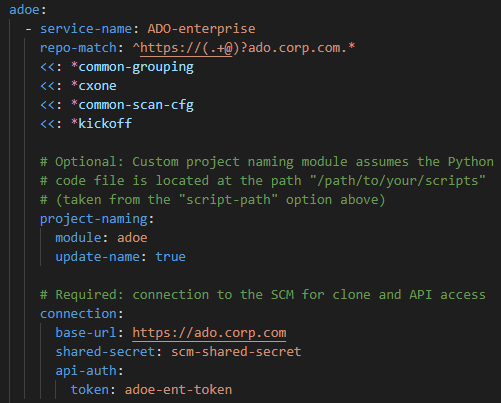
\includegraphics[width=\textwidth]{graphics/naming_example_adoe.png}
    \caption{Azure DevOps Custom Project Naming YAML Configuration}
    \label{fig:naming-yaml-adoe}
\end{figure}


\begin{figure}[h]
    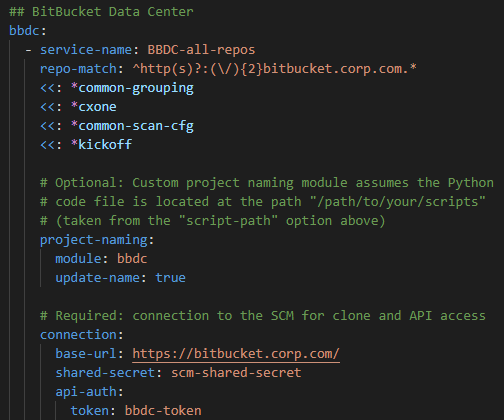
\includegraphics[width=\textwidth]{graphics/naming_example_bbdc.png}
    \caption{BitBucket Data Center Custom Project Naming YAML Configuration}
    \label{fig:naming-yaml-bbdc}
\end{figure}

\begin{figure}[h]
    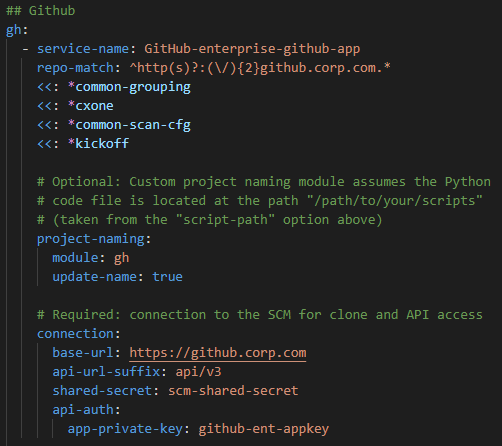
\includegraphics[width=\textwidth]{graphics/naming_example_gh.png}
    \caption{GitHub Custom Project Naming YAML Configuration}
    \label{fig:naming-yaml-gh}
\end{figure}

\begin{figure}[h]
    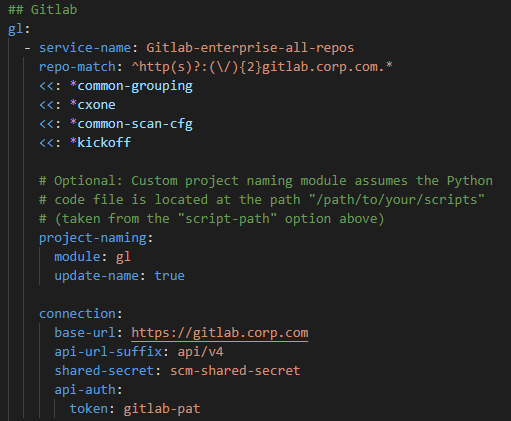
\includegraphics[width=\textwidth]{graphics/naming_example_gl.png}
    \caption{Gitlab Custom Project Naming YAML Configuration}
    \label{fig:naming-yaml-gl}
\end{figure}

When the naming script executes, any errors will assign the default project name to the project.  
The \texttt{project-naming.update-name} configuration element in the YAML examples is set to \texttt{True}.  This indicates that
projects previously created with a default project name, if found, will be renamed with the dynamic project name.  This
renaming activity occurs only upon handling an event generated by a push or pull-request for the corresponding
repository.  If \texttt{project-naming.update-name} is set to \texttt{False} and a project with the default name
is found when handling an event, the existing project is used when starting the scan.


\section{Name Selection Logic}

Dynamic project naming is a transformation activity to take data elements from an SCM-generated event and yield
a project name with those elements.  The default project name convention follows the SCM repository organization
scheme and thus varies by SCM.  If \cxoneflow is configured to handle events generated from more than one SCM type,
it should be expected that a dynamic naming script would be required for each configured SCM type.

In the absence of a dynamic project naming configuration, default project names will be used.

When an event is handled by \cxoneflow and dynamic project naming is configured, the following logic is applied
to select the project name selected for the scan:

\begin{enumerate}
  \item If neither the dynamic project name or default project name exists, a new project with the dynamic project name is created.
  \item If the dynamic project name exists, it is selected.
  \item If the dynamic project name does not exist:
  \begin{enumerate}
    \item If \texttt{project-naming.update-name} is \texttt{True}, the default project is renamed using the dynamic project name
    and the dynamic project name is selected.
    \item If \texttt{project-naming.update-name} is \texttt{False}, the default project name is selected.
  \end{enumerate}
\end{enumerate}

Adding a configuration for dynamic project names in a system that has been operational will not alter scan history
for any projects.  Depending on configuration options, projects can be renamed but will retain all other aspects
of the project prior to the name change.


\section{Implementation Guidelines}

Python is a general purpose programming language that allows nearly unlimited possibilities for what is
executed upon invocation of the dynamic project naming module.  The intention of this feature is not, however,
to act as a general purpose integration point.  Dynamic project naming scripts that execute outside of the
guidelines in this section is considered out-of-scope for any supportability.

\subsection{Execution Time}

The intention of the dynamic project naming feature is to provide the ability to extract data from the
event and/or the SCM associated with the service definition handling the event.  As such, the
average execution time of a dynamic project naming script should be less than 1 second.

\subsection{Additional Third-Party Python Modules}

Adding additional Python modules beyond what is used by \cxoneflow is considered out-of-scope.

\subsection{Local File Access}

While it is possible to perform local file access via Python built-in libraries, doing so
is considered out-of-scope.

\subsection{Statelessness}

Maintaining any in-memory state in across invocations of a dynamic project naming script is considered out-of-scope.
If the implementation requires maintaining state through using external services, it should be done so within the
execution time guidelines.

\subsection{Robustness of Implementation}

It is assumed that the implementation of a dynamic project naming script is robust given dynamic project naming scripts
are intended to be simple implementations.  A dynamic projecting naming script that fails with an exception, returning \texttt{None} due to an error
condition, or returns the same name for multiple repositories will cause scans to be created in incorrect projects.  If
a dynamic project naming script is failing with high frequency, consider simplifying the implementation.

Intermittent failures of the dynamic naming script may cause projects with the default name to appear when the dynamic
naming script fails to execute properly.  Scripts that use the SCM API, for example, may occasionally see an error
response when attempting to use the SCM's API.  The dynamic naming script should be resilient to temporary issues
accessing the SCM API.  Keep in mind that coding around system failures due to an instable system can only go so
far before the remote system's instability problems must be remediated to ensure reliability.

If the dynamic script failures due to SCM instability are impacting the use of the dynamic naming feature, the
only recourse will be to simplify the implementation such that contact with the SCM's APIs are not required.


\section{Authoring Dynamic Project Naming Scripts}

\subsection{Security Warning}

The dynamic project naming scripts that execute in \cxoneflow are written in Python with execution in the context of
the \cxoneflow daemon process.  Given that Python is a general purpose programming language, anything that can be executed
as a running Python program can be executed during the dynamic project name module execution.  Care should be taken to
prevent the content of the dynamic project naming scripts from being modified by unauthorized individuals.

\subsection{Dynamic Project Naming API Implementation}

A dynamic project naming module must implement a single method named \texttt{event\_project\_name\_factory}. The code
listing below shows the prototype of \texttt{event\_project\_name\_factory}:

\begin{code}{Dynamic Project Naming Method Prototype}{}{}
async def event_project_name_factory(context : EventContext, scm_service : BasicSCMService) -> str : ...
\end{code}

\cxoneflow will invoke the instance of \texttt{event\_project\_name\_factory} when orchestrating a scan and expect
it to return a string value for the dynamic project name.  If \texttt{event\_project\_name\_factory} returns \texttt{None}
or throws an exception, the default project name is used.

\subsubsection{\texttt{EventContext} Parameter}

The \texttt{EventContext} parameter contains the elements of the event that caused a scan to be orchestrated.
The \texttt{EventContext.headers} property is a dictionary containing headers sent along with the event.  The
\texttt{EventContext.message} property is a dictionary containing the JSON content of the event.

The event message content can vary and guard code should be used to ensure interpretation of the event properly.
Events that orchestrate scans can be formed differently by the SCM for push and pull-request events.  Events may also
come from events received through the \intlink{sec:kickoff}{Kickoff} endpoints for each SCM.  The content for Kickoff
messages varies for each SCM type.

\subsubsection{\texttt{BasicSCMService} Parameter}

The \texttt{BasicSCMService} parameter is an object to allow for performing authenticated SCM API calls.  It is useful for
cases where additional information from the SCM API is needed to fully form the project name.  Performing API calls may
lead to long execution times for the dynamic project naming script.

\subsection{Debugging Dynamic Project Naming Scripts}

Debugging script execution with an IDE is possible using the techniques described in Appendix \ref{sec:cxoneflow-development}.
This loads \cxoneflow in a debug development mode which will allow setting breakpoints in the dynamic project naming code.

Another option is to use the Python built-in \texttt{logging} module.  Logging output from the dynamic naming script can be
observed along with any other logging output produced by \cxoneflowns.  Using the logging output, it is possible to track
execution logic and view the data stored in any variables.

\subsection{Example Dynamic Naming Script Code}

The example naming scripts in this section can be used as a starting point for creating your own
dynamic naming scripts.  The implementations are intended to show variations of naming scripts to
demonstrate how to adapt to naming requirements.

\pagebreak
\subsubsection{Azure DevOps Example}
The dynamic project naming script in the code listing for the \texttt{adoe}
code example is shown in Figure \ref{fig:naming-code-adoe}.  This is used to create a project with the naming convention:\\\\
\texttt{<first 6 or less chars of collection>\_<project name>\_<repo name>}\\

In this example, an authenticated API call is made to retrieve the collection name
for the collection id provided in the event context.

\begin{figure}[h]
    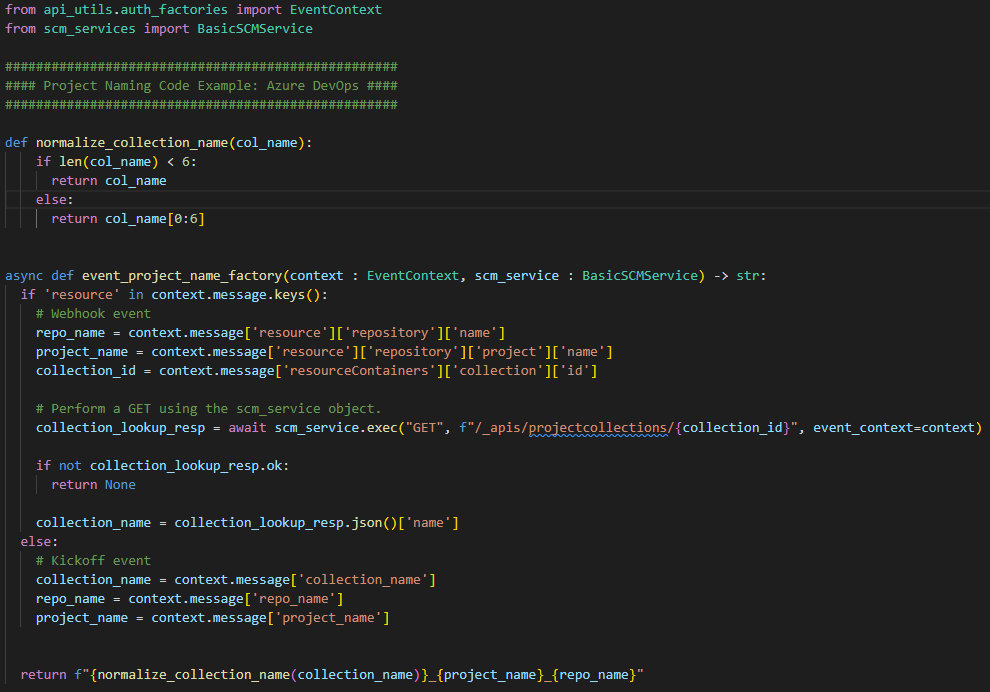
\includegraphics[width=\textwidth]{graphics/naming-code-adoe.png}
    \caption{Azure DevOps Custom Project Naming Code Example}
    \label{fig:naming-code-adoe}
\end{figure}


\pagebreak
\subsubsection{BitBucket Data Center Example}
Figure \ref{fig:naming-code-bbdc} shows the listing for the \texttt{bbdc} code example creates a project name from
the event context in the format of \texttt{<project key>\_<repository name>}:

\begin{figure}[h]
    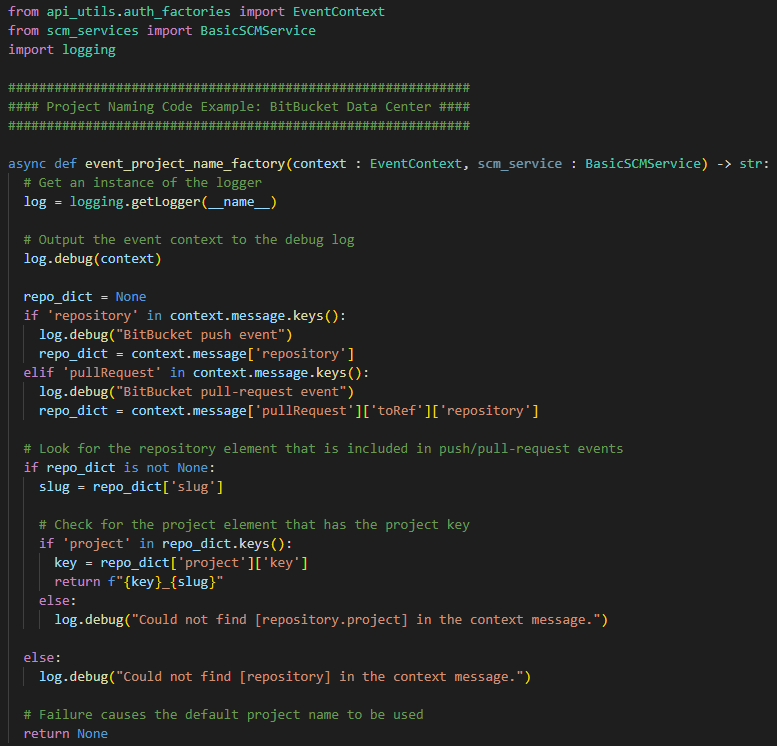
\includegraphics[width=\textwidth]{graphics/naming-code-bbdc.png}
    \caption{BitBucket Data Center Custom Project Naming Code Example}
    \label{fig:naming-code-bbdc}
\end{figure}


\pagebreak
\subsubsection{GitHub Example}
The dynamic project naming script in the code listing for the \texttt{gh}
code example is shown In Figure \ref{fig:naming-code-gh}.  This is used to create a project with the naming convention:\\\\
\texttt{<first 6 or less chars of organization>\_<repo name>}\\

\begin{figure}[h]
    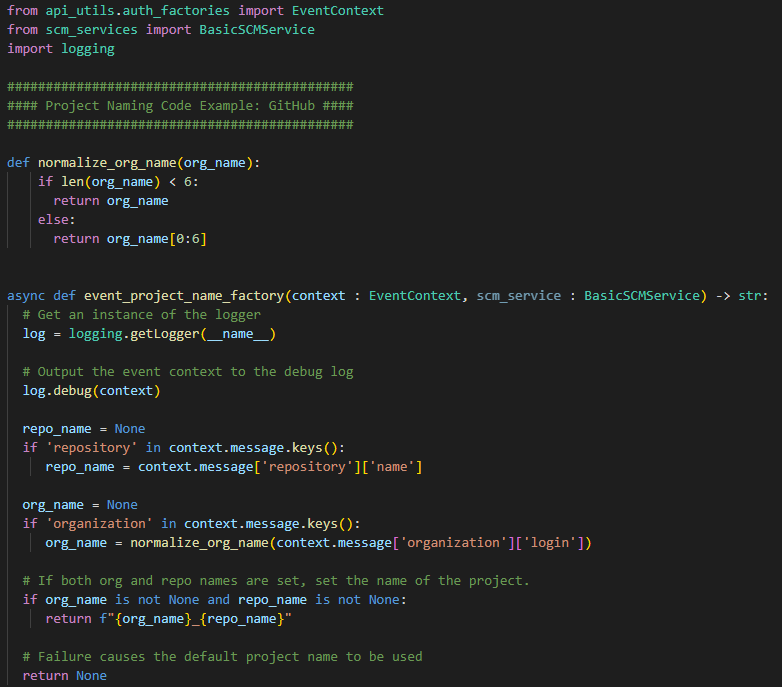
\includegraphics[width=\textwidth]{graphics/naming-code-gh.png}
    \caption{GitHub Custom Project Naming Code Example}
    \label{fig:naming-code-gh}
\end{figure}


\pagebreak
\subsubsection{Gitlab Example}
The dynamic project naming script in the code listing for the \texttt{gl}
code example is shown in Figure \ref{fig:naming-code-gl}.  This changes the naming convention of the projects to create
a path containing only the upper-case characters in the namespace path and to use
the project's full name at the end of the abbreviated namespace path.

The example utilizes the SCM's API to get the project details that are not included
with the webhook event payload.\\

\begin{figure}[h]
    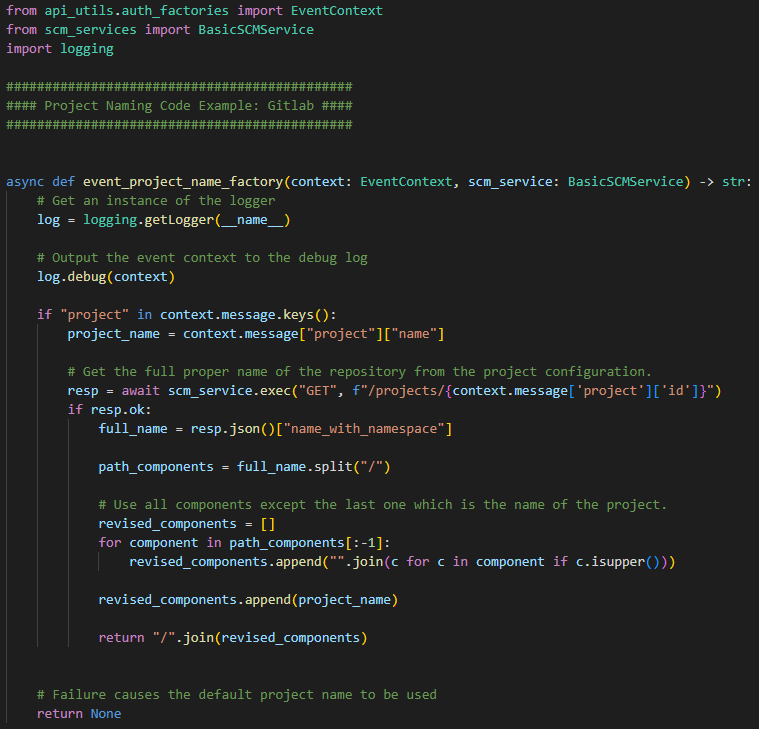
\includegraphics[width=\textwidth]{graphics/naming-code-gl.png}
    \caption{Gitlab Custom Project Naming Code Example}
    \label{fig:naming-code-gl}
\end{figure}




